\documentclass[twoside]{book}

% Packages required by doxygen
\usepackage{fixltx2e}
\usepackage{calc}
\usepackage{doxygen}
\usepackage[export]{adjustbox} % also loads graphicx
\usepackage{graphicx}
\usepackage[utf8]{inputenc}
\usepackage{makeidx}
\usepackage{multicol}
\usepackage{multirow}
\PassOptionsToPackage{warn}{textcomp}
\usepackage{textcomp}
\usepackage[nointegrals]{wasysym}
\usepackage[table]{xcolor}

% Font selection
\usepackage[T1]{fontenc}
\usepackage[scaled=.90]{helvet}
\usepackage{courier}
\usepackage{amssymb}
\usepackage{sectsty}
\renewcommand{\familydefault}{\sfdefault}
\allsectionsfont{%
  \fontseries{bc}\selectfont%
  \color{darkgray}%
}
\renewcommand{\DoxyLabelFont}{%
  \fontseries{bc}\selectfont%
  \color{darkgray}%
}
\newcommand{\+}{\discretionary{\mbox{\scriptsize$\hookleftarrow$}}{}{}}

% Page & text layout
\usepackage{geometry}
\geometry{%
  a4paper,%
  top=2.5cm,%
  bottom=2.5cm,%
  left=2.5cm,%
  right=2.5cm%
}
\tolerance=750
\hfuzz=15pt
\hbadness=750
\setlength{\emergencystretch}{15pt}
\setlength{\parindent}{0cm}
\setlength{\parskip}{3ex plus 2ex minus 2ex}
\makeatletter
\renewcommand{\paragraph}{%
  \@startsection{paragraph}{4}{0ex}{-1.0ex}{1.0ex}{%
    \normalfont\normalsize\bfseries\SS@parafont%
  }%
}
\renewcommand{\subparagraph}{%
  \@startsection{subparagraph}{5}{0ex}{-1.0ex}{1.0ex}{%
    \normalfont\normalsize\bfseries\SS@subparafont%
  }%
}
\makeatother

% Headers & footers
\usepackage{fancyhdr}
\pagestyle{fancyplain}
\fancyhead[LE]{\fancyplain{}{\bfseries\thepage}}
\fancyhead[CE]{\fancyplain{}{}}
\fancyhead[RE]{\fancyplain{}{\bfseries\leftmark}}
\fancyhead[LO]{\fancyplain{}{\bfseries\rightmark}}
\fancyhead[CO]{\fancyplain{}{}}
\fancyhead[RO]{\fancyplain{}{\bfseries\thepage}}
\fancyfoot[LE]{\fancyplain{}{}}
\fancyfoot[CE]{\fancyplain{}{}}
\fancyfoot[RE]{\fancyplain{}{\bfseries\scriptsize Generated by Doxygen }}
\fancyfoot[LO]{\fancyplain{}{\bfseries\scriptsize Generated by Doxygen }}
\fancyfoot[CO]{\fancyplain{}{}}
\fancyfoot[RO]{\fancyplain{}{}}
\renewcommand{\footrulewidth}{0.4pt}
\renewcommand{\chaptermark}[1]{%
  \markboth{#1}{}%
}
\renewcommand{\sectionmark}[1]{%
  \markright{\thesection\ #1}%
}

% Indices & bibliography
\usepackage{natbib}
\usepackage[titles]{tocloft}
\setcounter{tocdepth}{3}
\setcounter{secnumdepth}{5}
\makeindex

% Hyperlinks (required, but should be loaded last)
\usepackage{ifpdf}
\ifpdf
  \usepackage[pdftex,pagebackref=true]{hyperref}
\else
  \usepackage[ps2pdf,pagebackref=true]{hyperref}
\fi
\hypersetup{%
  colorlinks=true,%
  linkcolor=blue,%
  citecolor=blue,%
  unicode%
}

% Custom commands
\newcommand{\clearemptydoublepage}{%
  \newpage{\pagestyle{empty}\cleardoublepage}%
}

\usepackage{caption}
\captionsetup{labelsep=space,justification=centering,font={bf},singlelinecheck=off,skip=4pt,position=top}

%===== C O N T E N T S =====

\begin{document}

% Titlepage & ToC
\hypersetup{pageanchor=false,
             bookmarksnumbered=true,
             pdfencoding=unicode
            }
\pagenumbering{alph}
\begin{titlepage}
\vspace*{7cm}
\begin{center}%
{\Large Transient dynamics in non-\/equilibrium complex systems \\[1ex]\large 1.\+0.\+0 }\\
\vspace*{1cm}
{\large Generated by Doxygen 1.8.13}\\
\end{center}
\end{titlepage}
\clearemptydoublepage
\pagenumbering{roman}
\tableofcontents
\clearemptydoublepage
\pagenumbering{arabic}
\hypersetup{pageanchor=true}

%--- Begin generated contents ---
\chapter{Transient dynamics in non-\/equilibrium complex systems}
\label{index}\hypertarget{index}{}\begin{center}\end{center} 

\begin{center}\tabulinesep=1mm
\begin{longtabu} spread 0pt [c]{*{2}{|X[-1]}|}
\hline
\rowcolor{\tableheadbgcolor}\textbf{ Gas Mixing Model }&\textbf{ Game Of Life  }\\\cline{1-2}
\endfirsthead
\hline
\endfoot
\hline
\rowcolor{\tableheadbgcolor}\textbf{ Gas Mixing Model }&\textbf{ Game Of Life  }\\\cline{1-2}
\endhead
 & \\\cline{1-2}
\end{longtabu}
\end{center} 





Simulation and analysis of transient dynamics in complex systems.

Code on github\+: \href{https://github.com/sellisd/transientDynamics}{\tt https\+://github.\+com/sellisd/transient\+Dynamics}

preprint at O\+SF\+: Sellis, D. (2018, July 26). Transient dynamics in non-\/equilibrium complex systems. Retrieved from \href{https://osf.io/bkz52/}{\tt https\+://osf.\+io/bkz52/}

\subsection*{Requirements}

\subsubsection*{transient\+Dynamics simulator}


\begin{DoxyItemize}
\item a C++ compiler such one of the following\+:
\begin{DoxyItemize}
\item g++ G\+NU Compiler Collection \href{https://gcc.gnu.org/}{\tt https\+://gcc.\+gnu.\+org/} or
\item clang \href{https://clang.llvm.org/}{\tt https\+://clang.\+llvm.\+org/}
\end{DoxyItemize}
\end{DoxyItemize}

\subsubsection*{Analysis of results}


\begin{DoxyItemize}
\item R \href{https://www.r-project.org/}{\tt https\+://www.\+r-\/project.\+org/}
\end{DoxyItemize}

\subsubsection*{Running a simulations}

Once all requirements are satisfied compile the source with


\begin{DoxyCode}
$> cd src
$> make
\end{DoxyCode}


A file {\ttfamily run} is generated that be used to launch a simulation\+:


\begin{DoxyCode}
./run side model replicates Tmax byS byW byV statisticsFile windowFile vectorFile

where:

side:           int       The side of the world matrix

model           [1,2,3,4] The model to simulate:
                            1:     Gas mixing
                            2:     Game of Life
                            3:     Gradient
                            4:     Uniform

replicates      int       How many simulations to run

Tmax            int       Number of cycles to run

byS             int       Save output file statisticsFile every byS cycles

byW             int       Save output file windowFile every byS cycles

byV             int       Save output file vectorFile every byS cycles

statisticsFile  string    Path and filename for statistics output file. This
                          file contains summary statistics for each cycle

windowFile      string    Path and filename for window output file. This file
                          contains summary statistics for each cycle and coarse
                          graining window size

vectorFile      string    Path and filename for vector output file. This file
                          contains world matrix concatenated to a vector for
                          each cycle
\end{DoxyCode}


\subsubsection*{Output file format}

\paragraph*{Statistics output file}

The statistics output file is a tab separated file that has information for each cycle (one cycle per row) with the following columns\+:

\tabulinesep=1mm
\begin{longtabu} spread 0pt [c]{*{2}{|X[-1]}|}
\hline
\rowcolor{\tableheadbgcolor}\textbf{ Name }&\textbf{ Description  }\\\cline{1-2}
\endfirsthead
\hline
\endfoot
\hline
\rowcolor{\tableheadbgcolor}\textbf{ Name }&\textbf{ Description  }\\\cline{1-2}
\endhead
replicate &Number of replicate simulation \\\cline{1-2}
generation&Cycle number \\\cline{1-2}
Ktl &Kolmogorov complexity of the top-\/left subregion of the system \\\cline{1-2}
Kce &Kolmogorov complexity of center subregion of the system \\\cline{1-2}
Kbr &Kolmogorov complexity of bottom-\/right subregion of the system \\\cline{1-2}
Htl &Information entropy of the top-\/left sybregion of the system \\\cline{1-2}
Hce &Information entropy of the center subregion of the system \\\cline{1-2}
Hbr &Information entropy of the bottom-\/right subregion of the system \\\cline{1-2}
Dtl &Density of the top-\/left subregion of the system \\\cline{1-2}
Dce &Density of the center subregion of the system \\\cline{1-2}
Dbr &Density of the bottom-\/right subregion of the system \\\cline{1-2}
\end{longtabu}
\paragraph*{Window output file}

The window file is a tab delimited file that contains the output for each coarse graining window size

\tabulinesep=1mm
\begin{longtabu} spread 0pt [c]{*{2}{|X[-1]}|}
\hline
\rowcolor{\tableheadbgcolor}\textbf{ Name }&\textbf{ Description  }\\\cline{1-2}
\endfirsthead
\hline
\endfoot
\hline
\rowcolor{\tableheadbgcolor}\textbf{ Name }&\textbf{ Description  }\\\cline{1-2}
\endhead
replicate &Number of replicate simulation \\\cline{1-2}
generation&Cycle number \\\cline{1-2}
window &Size of coarse graining window \\\cline{1-2}
K &Kolmogorov complexity \\\cline{1-2}
H &Information entropy \\\cline{1-2}
S &Box counting dimension \\\cline{1-2}
\end{longtabu}
\paragraph*{Vector output file}

The vector output file contains has in each row the cycle number and the world matrix concatenated into a vector (space delimited) 
\chapter{Hierarchical Index}
\section{Class Hierarchy}
This inheritance list is sorted roughly, but not completely, alphabetically\+:\begin{DoxyCompactList}
\item \contentsline{section}{entropy}{\pageref{classentropy}}{}
\item \contentsline{section}{randomv}{\pageref{classrandomv}}{}
\item \contentsline{section}{system}{\pageref{classsystem}}{}
\begin{DoxyCompactList}
\item \contentsline{section}{game\+Of\+Life}{\pageref{classgame_of_life}}{}
\item \contentsline{section}{gas\+Mixing}{\pageref{classgas_mixing}}{}
\end{DoxyCompactList}
\end{DoxyCompactList}

\chapter{Class Index}
\section{Class List}
Here are the classes, structs, unions and interfaces with brief descriptions\+:\begin{DoxyCompactList}
\item\contentsline{section}{\hyperlink{classentropy}{entropy} }{\pageref{classentropy}}{}
\item\contentsline{section}{\hyperlink{classgame_of_life}{game\+Of\+Life} }{\pageref{classgame_of_life}}{}
\item\contentsline{section}{\hyperlink{classgas_mixing}{gas\+Mixing} }{\pageref{classgas_mixing}}{}
\item\contentsline{section}{\hyperlink{classrandomv}{randomv} \\*Random variable class }{\pageref{classrandomv}}{}
\item\contentsline{section}{\hyperlink{classsystem}{system} }{\pageref{classsystem}}{}
\end{DoxyCompactList}

\chapter{Class Documentation}
\hypertarget{classentropy}{}\section{entropy Class Reference}
\label{classentropy}\index{entropy@{entropy}}


{\ttfamily \#include $<$entropy.\+h$>$}



Collaboration diagram for entropy\+:
\nopagebreak
\begin{figure}[H]
\begin{center}
\leavevmode
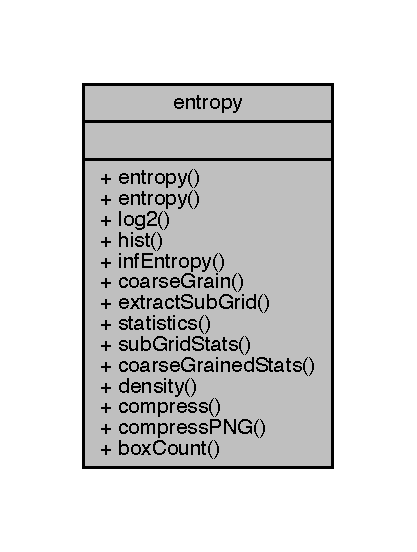
\includegraphics[width=200pt]{classentropy__coll__graph}
\end{center}
\end{figure}
\subsection*{Public Member Functions}
\begin{DoxyCompactItemize}
\item 
\mbox{\Hypertarget{classentropy_a669cc325fe3153318f31dd8008a28ca6}\label{classentropy_a669cc325fe3153318f31dd8008a28ca6}} 
\hyperlink{classentropy_a669cc325fe3153318f31dd8008a28ca6}{entropy} (int x, int y)
\begin{DoxyCompactList}\small\item\em Default constructor. \end{DoxyCompactList}\item 
\mbox{\Hypertarget{classentropy_adeae61cb4c6a7f89f80878adcd476f43}\label{classentropy_adeae61cb4c6a7f89f80878adcd476f43}} 
double \hyperlink{classentropy_adeae61cb4c6a7f89f80878adcd476f43}{log2} (double x)
\begin{DoxyCompactList}\small\item\em Constructor with size of grid. \end{DoxyCompactList}\item 
void \hyperlink{classentropy_a71fa5242cb3b25a8dc61e4fdd05ecf65}{hist} (map$<$ int, double $>$ \&, vector$<$ int $>$ \&vectorS)
\begin{DoxyCompactList}\small\item\em Calculate histogram of symbols. \end{DoxyCompactList}\item 
double \hyperlink{classentropy_a11cea34215fb0b30d0c5b1f97a4b2031}{inf\+Entropy} (map$<$ int, double $>$ \&\hyperlink{classentropy_a71fa5242cb3b25a8dc61e4fdd05ecf65}{hist})
\begin{DoxyCompactList}\small\item\em Calculate information entropy. \end{DoxyCompactList}\item 
void \hyperlink{classentropy_a1a52c035a25b949d699b8e17ffad8559}{coarse\+Grain} (vector$<$ int $>$ \&coarse\+Grained, int window, vector$<$ vector$<$ int $>$ $>$ \&grid)
\begin{DoxyCompactList}\small\item\em Coarse grain grid by summation. \end{DoxyCompactList}\item 
void \hyperlink{classentropy_a4dce3a1c33340db5371c2b5d4b64a62e}{extract\+Sub\+Grid} (vector$<$ vector$<$ int $>$ $>$ \&grid, vector$<$ int $>$ \&subgrid, int width, int x, int y)
\begin{DoxyCompactList}\small\item\em Extract a square region of the grid. \end{DoxyCompactList}\item 
void \hyperlink{classentropy_af3108d7ce02d1c592f283f117c0fe63f}{statistics} (vector$<$ int $>$ \&sub\+Grid, int sub\+Grid\+Side, vector$<$ double $>$ \&results)
\begin{DoxyCompactList}\small\item\em Calculate statistics on a subgrid vector. \end{DoxyCompactList}\item 
void \hyperlink{classentropy_ad8fb5db1c5168d71ee3c1a4badaa1c55}{sub\+Grid\+Stats} (vector$<$ vector$<$ int $>$ $>$ \&grid, vector$<$ double $>$ \&topleft\+Stats, vector$<$ double $>$ \&center\+Stats, vector$<$ double $>$ \&bottomright\+Stats)
\begin{DoxyCompactList}\small\item\em Statistics of three subgrids. \end{DoxyCompactList}\item 
void \hyperlink{classentropy_a1b96c4450456728759e0c7a607eccd6a}{coarse\+Grained\+Stats} (vector$<$ vector$<$ int $>$ $>$ \&grid, map$<$ int, vector$<$ double $>$ $>$ \&cg\+Stats)
\begin{DoxyCompactList}\small\item\em Statistics on coarse grained grid. \end{DoxyCompactList}\item 
double \hyperlink{classentropy_ada553811d6bcfb5ecb88691822d07834}{density} (vector$<$ int $>$ \&subgrid)
\begin{DoxyCompactList}\small\item\em Calculate the density of a subgrid. \end{DoxyCompactList}\item 
double \hyperlink{classentropy_afaf6890a65cab96d6f8ff6416f18a540}{compress} (vector$<$ int $>$ \&vectorS)
\begin{DoxyCompactList}\small\item\em Perform run length encoding compression. \end{DoxyCompactList}\item 
double \hyperlink{classentropy_afceb0407962f4114cae68d6f70dfb3ec}{compress\+P\+NG} (vector$<$ int $>$ \&vectorS, unsigned int window)
\begin{DoxyCompactList}\small\item\em Perform P\+NG compression on a std vector representing a square matrix. \end{DoxyCompactList}\item 
int \hyperlink{classentropy_a253fbd96c15371d3a19658c62a87bcc8}{box\+Count} (vector$<$ int $>$ \&vectorS)
\begin{DoxyCompactList}\small\item\em Calculate the box-\/counting dimension of a coarse grained vector. \end{DoxyCompactList}\end{DoxyCompactItemize}


\subsection{Detailed Description}
Entropy calculations 

Definition at line 8 of file entropy.\+h.



\subsection{Member Function Documentation}
\mbox{\Hypertarget{classentropy_a253fbd96c15371d3a19658c62a87bcc8}\label{classentropy_a253fbd96c15371d3a19658c62a87bcc8}} 
\index{entropy@{entropy}!box\+Count@{box\+Count}}
\index{box\+Count@{box\+Count}!entropy@{entropy}}
\subsubsection{\texorpdfstring{box\+Count()}{boxCount()}}
{\footnotesize\ttfamily int entropy\+::box\+Count (\begin{DoxyParamCaption}\item[{vector$<$ int $>$ \&}]{vectorS }\end{DoxyParamCaption})}



Calculate the box-\/counting dimension of a coarse grained vector. 

Calculate box counting dimension (Minkowski-\/\+Bouligand). As the input is already coarse grained we just have to calculate the sum of entries $>$ 0 
\begin{DoxyParams}[1]{Parameters}
\mbox{\tt in}  & {\em vectorS} & Coarse grained vector. \\
\hline
\end{DoxyParams}
\begin{DoxyReturn}{Returns}
int Box counting dimension 
\end{DoxyReturn}


Definition at line 190 of file entropy.\+cpp.

\mbox{\Hypertarget{classentropy_a1a52c035a25b949d699b8e17ffad8559}\label{classentropy_a1a52c035a25b949d699b8e17ffad8559}} 
\index{entropy@{entropy}!coarse\+Grain@{coarse\+Grain}}
\index{coarse\+Grain@{coarse\+Grain}!entropy@{entropy}}
\subsubsection{\texorpdfstring{coarse\+Grain()}{coarseGrain()}}
{\footnotesize\ttfamily void entropy\+::coarse\+Grain (\begin{DoxyParamCaption}\item[{vector$<$ int $>$ \&}]{coarse\+Grained,  }\item[{int}]{window,  }\item[{vector$<$ vector$<$ int $>$ $>$ \&}]{grid }\end{DoxyParamCaption})}



Coarse grain grid by summation. 

Non overlapping windows of side window are used to cover the whole grid and within each window the sum of all cell values is calculated. There is no checks for errors, so x and y should always be powers of 2. 
\begin{DoxyParams}[1]{Parameters}
\mbox{\tt out}  & {\em coarse\+Grained} & One dimensional vector of coarse grained grid. \\
\hline
\mbox{\tt in}  & {\em window} & Side of window for coarse graining. \\
\hline
\mbox{\tt in}  & {\em grid} & Grid of system. \\
\hline
\end{DoxyParams}
\begin{DoxyReturn}{Returns}
Nothing. 
\end{DoxyReturn}


Definition at line 103 of file entropy.\+cpp.

\mbox{\Hypertarget{classentropy_a1b96c4450456728759e0c7a607eccd6a}\label{classentropy_a1b96c4450456728759e0c7a607eccd6a}} 
\index{entropy@{entropy}!coarse\+Grained\+Stats@{coarse\+Grained\+Stats}}
\index{coarse\+Grained\+Stats@{coarse\+Grained\+Stats}!entropy@{entropy}}
\subsubsection{\texorpdfstring{coarse\+Grained\+Stats()}{coarseGrainedStats()}}
{\footnotesize\ttfamily void entropy\+::coarse\+Grained\+Stats (\begin{DoxyParamCaption}\item[{vector$<$ vector$<$ int $>$ $>$ \&}]{grid,  }\item[{map$<$ int, vector$<$ double $>$ $>$ \&}]{cg\+Stats }\end{DoxyParamCaption})}



Statistics on coarse grained grid. 

Coarse grain the system\textquotesingle{}s grid at different scales with non-\/overlapping windows of size $w = 1^i$, with $i \in (1, 2, 3, 4, 5, 6)$ and for each window size calculate statistics. 
\begin{DoxyParams}[1]{Parameters}
\mbox{\tt in}  & {\em grid} & Grid of the system. \\
\hline
\mbox{\tt out}  & {\em cg\+Stats} & Statistics for each coarse graining window size. \\
\hline
\end{DoxyParams}
\begin{DoxyReturn}{Returns}
Nothing 
\end{DoxyReturn}


Definition at line 79 of file entropy.\+cpp.

\mbox{\Hypertarget{classentropy_afaf6890a65cab96d6f8ff6416f18a540}\label{classentropy_afaf6890a65cab96d6f8ff6416f18a540}} 
\index{entropy@{entropy}!compress@{compress}}
\index{compress@{compress}!entropy@{entropy}}
\subsubsection{\texorpdfstring{compress()}{compress()}}
{\footnotesize\ttfamily double entropy\+::compress (\begin{DoxyParamCaption}\item[{vector$<$ int $>$ \&}]{vectorS }\end{DoxyParamCaption})}



Perform run length encoding compression. 

Compress vector with a run length encoding list, e.\+g.\+: 000111002 -\/$>$ 03130221. 
\begin{DoxyParams}[1]{Parameters}
\mbox{\tt in}  & {\em vectorS} & Vector to compress \\
\hline
\end{DoxyParams}
\begin{DoxyReturn}{Returns}
Size of compressed vector. 
\end{DoxyReturn}


Definition at line 119 of file entropy.\+cpp.

\mbox{\Hypertarget{classentropy_afceb0407962f4114cae68d6f70dfb3ec}\label{classentropy_afceb0407962f4114cae68d6f70dfb3ec}} 
\index{entropy@{entropy}!compress\+P\+NG@{compress\+P\+NG}}
\index{compress\+P\+NG@{compress\+P\+NG}!entropy@{entropy}}
\subsubsection{\texorpdfstring{compress\+P\+N\+G()}{compressPNG()}}
{\footnotesize\ttfamily double entropy\+::compress\+P\+NG (\begin{DoxyParamCaption}\item[{vector$<$ int $>$ \&}]{vectorS,  }\item[{unsigned int}]{window }\end{DoxyParamCaption})}



Perform P\+NG compression on a std vector representing a square matrix. 

Uses lodepng to perform a P\+NG compression to a std vector which represents a square matrix. 
\begin{DoxyParams}[1]{Parameters}
\mbox{\tt in}  & {\em vectorS} & Vector to compress \\
\hline
\mbox{\tt in}  & {\em window} & Side of the square matrix \\
\hline
\end{DoxyParams}
\begin{DoxyReturn}{Returns}
Nothing 
\end{DoxyReturn}


Definition at line 145 of file entropy.\+cpp.

\mbox{\Hypertarget{classentropy_ada553811d6bcfb5ecb88691822d07834}\label{classentropy_ada553811d6bcfb5ecb88691822d07834}} 
\index{entropy@{entropy}!density@{density}}
\index{density@{density}!entropy@{entropy}}
\subsubsection{\texorpdfstring{density()}{density()}}
{\footnotesize\ttfamily double entropy\+::density (\begin{DoxyParamCaption}\item[{vector$<$ int $>$ \&}]{subgrid }\end{DoxyParamCaption})}



Calculate the density of a subgrid. 

Calculates the ratio of occupied cells to total cells. 
\begin{DoxyParams}[1]{Parameters}
\mbox{\tt in}  & {\em subgrid} & The subgrid vector. \\
\hline
\end{DoxyParams}
\begin{DoxyReturn}{Returns}
The density of the region 
\end{DoxyReturn}


Definition at line 93 of file entropy.\+cpp.

\mbox{\Hypertarget{classentropy_a4dce3a1c33340db5371c2b5d4b64a62e}\label{classentropy_a4dce3a1c33340db5371c2b5d4b64a62e}} 
\index{entropy@{entropy}!extract\+Sub\+Grid@{extract\+Sub\+Grid}}
\index{extract\+Sub\+Grid@{extract\+Sub\+Grid}!entropy@{entropy}}
\subsubsection{\texorpdfstring{extract\+Sub\+Grid()}{extractSubGrid()}}
{\footnotesize\ttfamily void entropy\+::extract\+Sub\+Grid (\begin{DoxyParamCaption}\item[{vector$<$ vector$<$ int $>$ $>$ \&}]{grid,  }\item[{vector$<$ int $>$ \&}]{subgrid,  }\item[{int}]{width,  }\item[{int}]{x,  }\item[{int}]{y }\end{DoxyParamCaption})}



Extract a square region of the grid. 

Extracts a square region of the grid and returns it as a one dimensional vector. 
\begin{DoxyParams}[1]{Parameters}
\mbox{\tt in}  & {\em grid} & Grid of the systm. \\
\hline
\mbox{\tt out}  & {\em subgrid} & Extracted square. \\
\hline
\mbox{\tt in}  & {\em width} & Side of the square to extract. \\
\hline
 & {\em x} & Row index of top-\/left corner of subgrid \\
\hline
 & {\em y} & Column index of top-\/left corner of subgrid \\
\hline
\end{DoxyParams}
\begin{DoxyReturn}{Returns}
Nothing 
\end{DoxyReturn}


Definition at line 49 of file entropy.\+cpp.

\mbox{\Hypertarget{classentropy_a71fa5242cb3b25a8dc61e4fdd05ecf65}\label{classentropy_a71fa5242cb3b25a8dc61e4fdd05ecf65}} 
\index{entropy@{entropy}!hist@{hist}}
\index{hist@{hist}!entropy@{entropy}}
\subsubsection{\texorpdfstring{hist()}{hist()}}
{\footnotesize\ttfamily void entropy\+::hist (\begin{DoxyParamCaption}\item[{map$<$ int, double $>$ \&}]{hist,  }\item[{vector$<$ int $>$ \&}]{vectorS }\end{DoxyParamCaption})}



Calculate histogram of symbols. 

Base 2 logarithm Calculates the frequency of symbols in a vector of integers. 
\begin{DoxyParams}[1]{Parameters}
\mbox{\tt out}  & {\em hist} & Map of integer to double \\
\hline
\mbox{\tt in}  & {\em vectorS} & Symbol vector \\
\hline
\end{DoxyParams}
\begin{DoxyReturn}{Returns}
Nothing 
\end{DoxyReturn}


Definition at line 26 of file entropy.\+cpp.

\mbox{\Hypertarget{classentropy_a11cea34215fb0b30d0c5b1f97a4b2031}\label{classentropy_a11cea34215fb0b30d0c5b1f97a4b2031}} 
\index{entropy@{entropy}!inf\+Entropy@{inf\+Entropy}}
\index{inf\+Entropy@{inf\+Entropy}!entropy@{entropy}}
\subsubsection{\texorpdfstring{inf\+Entropy()}{infEntropy()}}
{\footnotesize\ttfamily double entropy\+::inf\+Entropy (\begin{DoxyParamCaption}\item[{map$<$ int, double $>$ \&}]{hist }\end{DoxyParamCaption})}



Calculate information entropy. 

Calculates the information entropy from a map of symbol frequencies. $H = -\sum_{k=1}^{p}\hat{\theta_k} log_2(\hat{\theta_k})$ 
\begin{DoxyParams}[1]{Parameters}
\mbox{\tt in}  & {\em hist} & Map of integer to double \\
\hline
\end{DoxyParams}
\begin{DoxyReturn}{Returns}
Information entropy in bits (log2) 
\end{DoxyReturn}


Definition at line 40 of file entropy.\+cpp.

\mbox{\Hypertarget{classentropy_af3108d7ce02d1c592f283f117c0fe63f}\label{classentropy_af3108d7ce02d1c592f283f117c0fe63f}} 
\index{entropy@{entropy}!statistics@{statistics}}
\index{statistics@{statistics}!entropy@{entropy}}
\subsubsection{\texorpdfstring{statistics()}{statistics()}}
{\footnotesize\ttfamily void entropy\+::statistics (\begin{DoxyParamCaption}\item[{vector$<$ int $>$ \&}]{sub\+Grid,  }\item[{int}]{sub\+Grid\+Side,  }\item[{vector$<$ double $>$ \&}]{results }\end{DoxyParamCaption})}



Calculate statistics on a subgrid vector. 

Calculates the Kolmogorov complexity, the information entropy and the density of non-\/zero cells on a subgrid vector. 
\begin{DoxyParams}[1]{Parameters}
\mbox{\tt in}  & {\em sub\+Grid} & Vector of subgrid. \\
\hline
\mbox{\tt in}  & {\em sub\+Grid\+Side} & Size of the square subgrid side. \\
\hline
\mbox{\tt out}  & {\em results} & Vector with results \mbox{[}K, H, D\mbox{]} \\
\hline
\end{DoxyParams}
\begin{DoxyReturn}{Returns}
Nothing. 
\end{DoxyReturn}


Definition at line 57 of file entropy.\+cpp.

\mbox{\Hypertarget{classentropy_ad8fb5db1c5168d71ee3c1a4badaa1c55}\label{classentropy_ad8fb5db1c5168d71ee3c1a4badaa1c55}} 
\index{entropy@{entropy}!sub\+Grid\+Stats@{sub\+Grid\+Stats}}
\index{sub\+Grid\+Stats@{sub\+Grid\+Stats}!entropy@{entropy}}
\subsubsection{\texorpdfstring{sub\+Grid\+Stats()}{subGridStats()}}
{\footnotesize\ttfamily void entropy\+::sub\+Grid\+Stats (\begin{DoxyParamCaption}\item[{vector$<$ vector$<$ int $>$ $>$ \&}]{grid,  }\item[{vector$<$ double $>$ \&}]{topleft\+Stats,  }\item[{vector$<$ double $>$ \&}]{center\+Stats,  }\item[{vector$<$ double $>$ \&}]{bottomright\+Stats }\end{DoxyParamCaption})}



Statistics of three subgrids. 

Calculate statistics at three square subgrids with side 8, the top left corner, the center and the bottom right. 
\begin{DoxyParams}[1]{Parameters}
\mbox{\tt in}  & {\em grid} & Grid of the system. \\
\hline
\mbox{\tt out}  & {\em topleft\+Stats} & Statistics for top left subgrid \\
\hline
\mbox{\tt out}  & {\em center\+Stats} & Statistics for center subgrid \\
\hline
\mbox{\tt out}  & {\em bottomright\+Stats} & Statistics for bottom right subgrid \\
\hline
\end{DoxyParams}
\begin{DoxyReturn}{Returns}
Nothing 
\end{DoxyReturn}


Definition at line 66 of file entropy.\+cpp.



The documentation for this class was generated from the following files\+:\begin{DoxyCompactItemize}
\item 
src/entropy.\+h\item 
src/entropy.\+cpp\end{DoxyCompactItemize}

\hypertarget{classgame_of_life}{}\section{game\+Of\+Life Class Reference}
\label{classgame_of_life}\index{game\+Of\+Life@{game\+Of\+Life}}


{\ttfamily \#include $<$game\+Of\+Life.\+h$>$}



Inheritance diagram for game\+Of\+Life\+:
\nopagebreak
\begin{figure}[H]
\begin{center}
\leavevmode
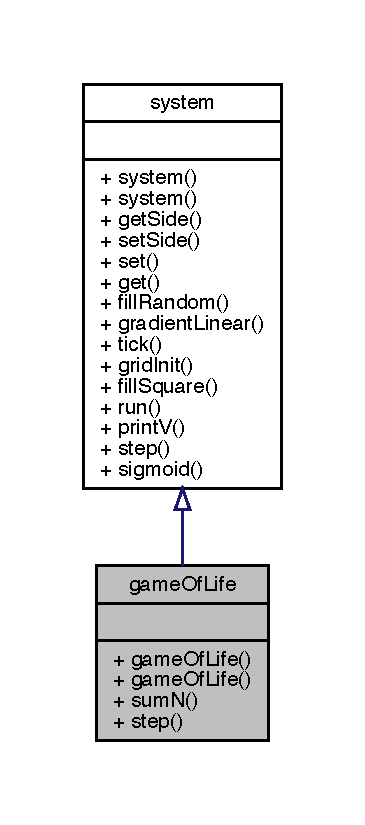
\includegraphics[width=175pt]{classgame_of_life__inherit__graph}
\end{center}
\end{figure}


Collaboration diagram for game\+Of\+Life\+:
\nopagebreak
\begin{figure}[H]
\begin{center}
\leavevmode
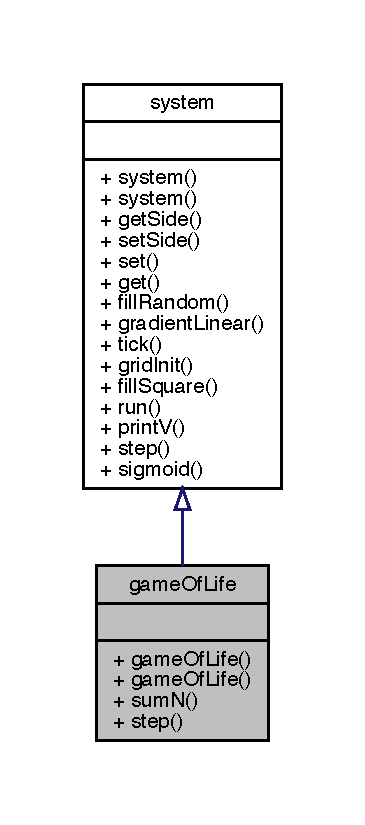
\includegraphics[width=175pt]{classgame_of_life__coll__graph}
\end{center}
\end{figure}
\subsection*{Public Member Functions}
\begin{DoxyCompactItemize}
\item 
\mbox{\Hypertarget{classgame_of_life_aa6b581822e3bc0ab045afebd7288d55e}\label{classgame_of_life_aa6b581822e3bc0ab045afebd7288d55e}} 
\hyperlink{classgame_of_life_aa6b581822e3bc0ab045afebd7288d55e}{game\+Of\+Life} (int side)
\begin{DoxyCompactList}\small\item\em Default constructor. \end{DoxyCompactList}\item 
int \hyperlink{classgame_of_life_a30febaa79f1e87d35b4eeae4f558fe13}{sumN} (int i, int j)
\begin{DoxyCompactList}\small\item\em Constructor with system side. \end{DoxyCompactList}\item 
\mbox{\Hypertarget{classgame_of_life_a7de2d57809b15f938ad18b8c30ddf9bf}\label{classgame_of_life_a7de2d57809b15f938ad18b8c30ddf9bf}} 
void \hyperlink{classgame_of_life_a7de2d57809b15f938ad18b8c30ddf9bf}{step} (\hyperlink{classrandomv}{randomv} \&r)
\begin{DoxyCompactList}\small\item\em Evolve the system by a single step. \end{DoxyCompactList}\end{DoxyCompactItemize}


\subsection{Detailed Description}
Game of Life on flat 2D torus grid 

Definition at line 14 of file game\+Of\+Life.\+h.



\subsection{Member Function Documentation}
\mbox{\Hypertarget{classgame_of_life_a30febaa79f1e87d35b4eeae4f558fe13}\label{classgame_of_life_a30febaa79f1e87d35b4eeae4f558fe13}} 
\index{game\+Of\+Life@{game\+Of\+Life}!sumN@{sumN}}
\index{sumN@{sumN}!game\+Of\+Life@{game\+Of\+Life}}
\subsubsection{\texorpdfstring{sum\+N()}{sumN()}}
{\footnotesize\ttfamily int game\+Of\+Life\+::sumN (\begin{DoxyParamCaption}\item[{int}]{i,  }\item[{int}]{j }\end{DoxyParamCaption})}



Constructor with system side. 

Calculate sum of values around cell i,j 
\begin{DoxyParams}[1]{Parameters}
\mbox{\tt in}  & {\em i} & x-\/axis coordinate. \\
\hline
\mbox{\tt in}  & {\em j} & y-\/axis coordinate. \\
\hline
\end{DoxyParams}
\begin{DoxyReturn}{Returns}
sum 
\end{DoxyReturn}


Definition at line 11 of file game\+Of\+Life.\+cpp.



The documentation for this class was generated from the following files\+:\begin{DoxyCompactItemize}
\item 
src/game\+Of\+Life.\+h\item 
src/game\+Of\+Life.\+cpp\end{DoxyCompactItemize}

\hypertarget{classgas_mixing}{}\section{gas\+Mixing Class Reference}
\label{classgas_mixing}\index{gas\+Mixing@{gas\+Mixing}}


{\ttfamily \#include $<$gas\+Mixing.\+h$>$}



Inheritance diagram for gas\+Mixing\+:
\nopagebreak
\begin{figure}[H]
\begin{center}
\leavevmode
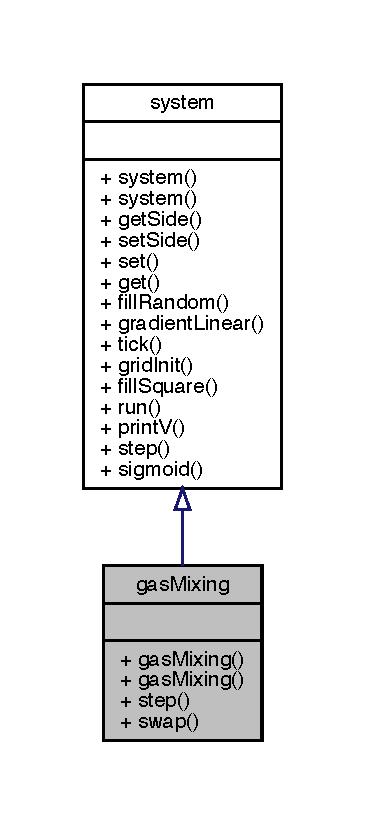
\includegraphics[width=175pt]{classgas_mixing__inherit__graph}
\end{center}
\end{figure}


Collaboration diagram for gas\+Mixing\+:
\nopagebreak
\begin{figure}[H]
\begin{center}
\leavevmode
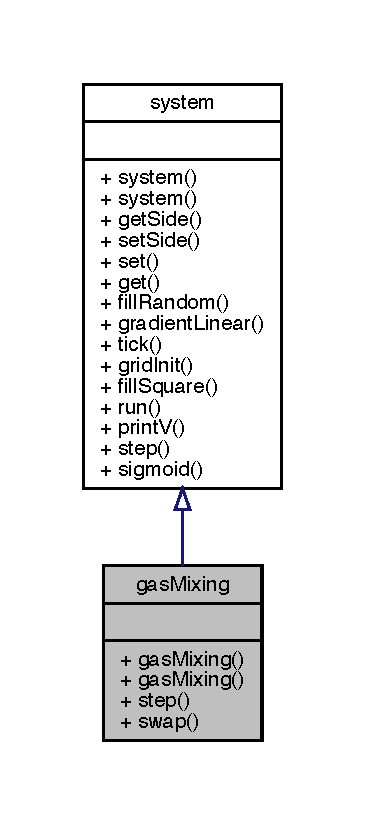
\includegraphics[width=175pt]{classgas_mixing__coll__graph}
\end{center}
\end{figure}
\subsection*{Public Member Functions}
\begin{DoxyCompactItemize}
\item 
\mbox{\Hypertarget{classgas_mixing_a5600907d75cc72807e733e34e6fae5b1}\label{classgas_mixing_a5600907d75cc72807e733e34e6fae5b1}} 
\hyperlink{classgas_mixing_a5600907d75cc72807e733e34e6fae5b1}{gas\+Mixing} (int side)
\begin{DoxyCompactList}\small\item\em Default constructor. \end{DoxyCompactList}\item 
void \hyperlink{classgas_mixing_acfd89f15487611dd77da9664642a06c6}{step} (\hyperlink{classrandomv}{randomv} \&r)
\begin{DoxyCompactList}\small\item\em Constructor with side of world. \end{DoxyCompactList}\item 
int \hyperlink{classgas_mixing_a99a14c1a13ee0ba938f4c1e22ad491b6}{swap} (int x1, int y1, int x2, int y2)
\end{DoxyCompactItemize}


\subsection{Detailed Description}
Gas mixing lattice rule is random swap two adjacent particles. At each time step, choose 2 horizontally or vertically adjacent squares uniformly at random and swap them only if they’re colored differentl 

Definition at line 18 of file gas\+Mixing.\+h.



\subsection{Member Function Documentation}
\mbox{\Hypertarget{classgas_mixing_acfd89f15487611dd77da9664642a06c6}\label{classgas_mixing_acfd89f15487611dd77da9664642a06c6}} 
\index{gas\+Mixing@{gas\+Mixing}!step@{step}}
\index{step@{step}!gas\+Mixing@{gas\+Mixing}}
\subsubsection{\texorpdfstring{step()}{step()}}
{\footnotesize\ttfamily void gas\+Mixing\+::step (\begin{DoxyParamCaption}\item[{\hyperlink{classrandomv}{randomv} \&}]{r }\end{DoxyParamCaption})\hspace{0.3cm}{\ttfamily [virtual]}}



Constructor with side of world. 

One time step (generation), extends the base class step. 
\begin{DoxyParams}[1]{Parameters}
\mbox{\tt in}  & {\em r} & Random number generation class. \\
\hline
\end{DoxyParams}
\begin{DoxyReturn}{Returns}
Nothing 
\end{DoxyReturn}


Reimplemented from \hyperlink{classsystem_aab28302f43e7ee42da51eb723f091533}{system}.



Definition at line 11 of file gas\+Mixing.\+cpp.

\mbox{\Hypertarget{classgas_mixing_a99a14c1a13ee0ba938f4c1e22ad491b6}\label{classgas_mixing_a99a14c1a13ee0ba938f4c1e22ad491b6}} 
\index{gas\+Mixing@{gas\+Mixing}!swap@{swap}}
\index{swap@{swap}!gas\+Mixing@{gas\+Mixing}}
\subsubsection{\texorpdfstring{swap()}{swap()}}
{\footnotesize\ttfamily int gas\+Mixing\+::swap (\begin{DoxyParamCaption}\item[{int}]{x1,  }\item[{int}]{y1,  }\item[{int}]{x2,  }\item[{int}]{y2 }\end{DoxyParamCaption})}

Move particle to new location if empty. 
\begin{DoxyParams}[1]{Parameters}
\mbox{\tt in}  & {\em x1} & X-\/axis coordinate of particle \\
\hline
\mbox{\tt in}  & {\em y1} & Y-\/axis coordinate of particle \\
\hline
\mbox{\tt in}  & {\em x2} & X-\/axis coordinate of target \\
\hline
\mbox{\tt in}  & {\em y2} & Y-\/axis coordinate of target \\
\hline
\end{DoxyParams}
\begin{DoxyReturn}{Returns}
int Movement performed (1) or not (0) 
\end{DoxyReturn}


Definition at line 42 of file gas\+Mixing.\+cpp.



The documentation for this class was generated from the following files\+:\begin{DoxyCompactItemize}
\item 
src/gas\+Mixing.\+h\item 
src/gas\+Mixing.\+cpp\end{DoxyCompactItemize}

\hypertarget{classrandomv}{}\section{randomv Class Reference}
\label{classrandomv}\index{randomv@{randomv}}


random variable class  




{\ttfamily \#include $<$randomv.\+h$>$}



Collaboration diagram for randomv\+:
\nopagebreak
\begin{figure}[H]
\begin{center}
\leavevmode
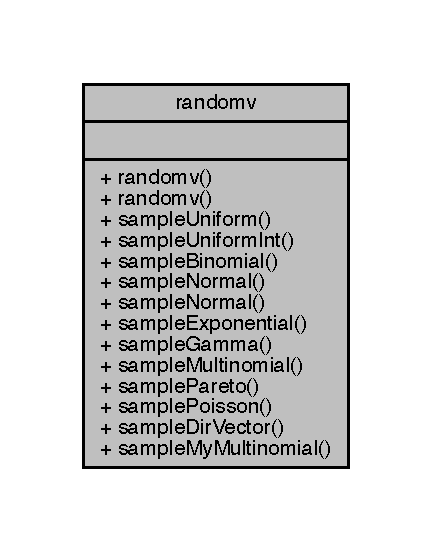
\includegraphics[width=207pt]{classrandomv__coll__graph}
\end{center}
\end{figure}
\subsection*{Public Member Functions}
\begin{DoxyCompactItemize}
\item 
\mbox{\Hypertarget{classrandomv_a32fc231d0bfb6a97c09d60fab19ed5fb}\label{classrandomv_a32fc231d0bfb6a97c09d60fab19ed5fb}} 
\hyperlink{classrandomv_a32fc231d0bfb6a97c09d60fab19ed5fb}{randomv} (void)
\begin{DoxyCompactList}\small\item\em constructor \end{DoxyCompactList}\item 
\hyperlink{classrandomv_a82d37b6df4f44746c5858578c265cd96}{randomv} (unsigned long seed)
\begin{DoxyCompactList}\small\item\em default constructor \end{DoxyCompactList}\item 
double \hyperlink{classrandomv_a0d1def37be5addf36b11234e3a7b29d3}{sample\+Uniform} (void)
\begin{DoxyCompactList}\small\item\em constructor with seed \end{DoxyCompactList}\item 
\mbox{\Hypertarget{classrandomv_a786b0ee6f4f4f4899326370a3112d4d8}\label{classrandomv_a786b0ee6f4f4f4899326370a3112d4d8}} 
int \hyperlink{classrandomv_a786b0ee6f4f4f4899326370a3112d4d8}{sample\+Uniform\+Int} (int n)
\begin{DoxyCompactList}\small\item\em sample from the uniform distribution $[0,1)$ \end{DoxyCompactList}\item 
\mbox{\Hypertarget{classrandomv_a7902b7016b5f9fb0b594e8575f8bf02a}\label{classrandomv_a7902b7016b5f9fb0b594e8575f8bf02a}} 
unsigned int \hyperlink{classrandomv_a7902b7016b5f9fb0b594e8575f8bf02a}{sample\+Binomial} (double p, int N)
\begin{DoxyCompactList}\small\item\em sample from the uniform distribution $[0,n-1)$ \end{DoxyCompactList}\item 
\mbox{\Hypertarget{classrandomv_aa8c9c4b22b274a3cc1d4d05f99a88f50}\label{classrandomv_aa8c9c4b22b274a3cc1d4d05f99a88f50}} 
double \hyperlink{classrandomv_aa8c9c4b22b274a3cc1d4d05f99a88f50}{sample\+Normal} (double mu, double sigma)
\begin{DoxyCompactList}\small\item\em sample from the binomial distribution \end{DoxyCompactList}\item 
double \hyperlink{classrandomv_a574eadd80c9cc66756c3417e55f2655c}{sample\+Normal} (double sigma)
\begin{DoxyCompactList}\small\item\em sample from a normal distribution with mean mu and standard deviation sigma \end{DoxyCompactList}\item 
double \hyperlink{classrandomv_afa56a12aa1bb44d7d4bd2a84303d9dca}{sample\+Exponential} (double mu)
\begin{DoxyCompactList}\small\item\em sample from a normal distribution with mean 0 and standard deviation sigma \end{DoxyCompactList}\item 
\mbox{\Hypertarget{classrandomv_a138a18fe2b991c0328510a7e077ca6a8}\label{classrandomv_a138a18fe2b991c0328510a7e077ca6a8}} 
double \hyperlink{classrandomv_a138a18fe2b991c0328510a7e077ca6a8}{sample\+Gamma} (double alpha, double beta)
\begin{DoxyCompactList}\small\item\em sample from an exponential distribution with mean mu \end{DoxyCompactList}\item 
\mbox{\Hypertarget{classrandomv_ab840593c1344749631c73321f589370f}\label{classrandomv_ab840593c1344749631c73321f589370f}} 
void \hyperlink{classrandomv_ab840593c1344749631c73321f589370f}{sample\+Multinomial} (size\+\_\+t K, unsigned int N, const double p\mbox{[}$\,$\mbox{]}, unsigned int n\mbox{[}$\,$\mbox{]})
\begin{DoxyCompactList}\small\item\em sample from a gamma distribution with parameters alpha and beta \end{DoxyCompactList}\item 
\mbox{\Hypertarget{classrandomv_a8973843ea2a27dc967333c712b89e788}\label{classrandomv_a8973843ea2a27dc967333c712b89e788}} 
double \hyperlink{classrandomv_a8973843ea2a27dc967333c712b89e788}{sample\+Pareto} (double alpha, double beta)
\begin{DoxyCompactList}\small\item\em sample from a pareto distribution with parameters alpha and beta $p(x) dx = (a/b) / (x/b)^{a+1} dx$ \end{DoxyCompactList}\item 
\mbox{\Hypertarget{classrandomv_a53890cf6d45e02337dbd348297f2901f}\label{classrandomv_a53890cf6d45e02337dbd348297f2901f}} 
double \hyperlink{classrandomv_a53890cf6d45e02337dbd348297f2901f}{sample\+Poisson} (double lambda)
\begin{DoxyCompactList}\small\item\em sample from Poisson distribution \end{DoxyCompactList}\item 
\mbox{\Hypertarget{classrandomv_a8739e952003183c95986dd2873058735}\label{classrandomv_a8739e952003183c95986dd2873058735}} 
void \hyperlink{classrandomv_a8739e952003183c95986dd2873058735}{sample\+Dir\+Vector} (int dimensions, size\+\_\+t n, double $\ast$x)
\begin{DoxyCompactList}\small\item\em sample random directional vector \end{DoxyCompactList}\item 
\mbox{\Hypertarget{classrandomv_ad9386cb5a1f8413515add301e707387f}\label{classrandomv_ad9386cb5a1f8413515add301e707387f}} 
int \hyperlink{classrandomv_ad9386cb5a1f8413515add301e707387f}{sample\+My\+Multinomial} (int Num\+Of\+Genotypes, unsigned int N, const double p\mbox{[}$\,$\mbox{]}, unsigned int new\+Generationp\mbox{[}$\,$\mbox{]})
\begin{DoxyCompactList}\small\item\em sample from multinomial function \end{DoxyCompactList}\end{DoxyCompactItemize}


\subsection{Detailed Description}
random variable class 

an object oriented interface for sampling from distributions using gsl 

Definition at line 9 of file randomv.\+h.



\subsection{Constructor \& Destructor Documentation}
\mbox{\Hypertarget{classrandomv_a82d37b6df4f44746c5858578c265cd96}\label{classrandomv_a82d37b6df4f44746c5858578c265cd96}} 
\index{randomv@{randomv}!randomv@{randomv}}
\index{randomv@{randomv}!randomv@{randomv}}
\subsubsection{\texorpdfstring{randomv()}{randomv()}}
{\footnotesize\ttfamily randomv\+::randomv (\begin{DoxyParamCaption}\item[{unsigned long}]{seed }\end{DoxyParamCaption})}



default constructor 

constructor with seed 

Definition at line 16 of file randomv.\+cpp.



\subsection{Member Function Documentation}
\mbox{\Hypertarget{classrandomv_afa56a12aa1bb44d7d4bd2a84303d9dca}\label{classrandomv_afa56a12aa1bb44d7d4bd2a84303d9dca}} 
\index{randomv@{randomv}!sample\+Exponential@{sample\+Exponential}}
\index{sample\+Exponential@{sample\+Exponential}!randomv@{randomv}}
\subsubsection{\texorpdfstring{sample\+Exponential()}{sampleExponential()}}
{\footnotesize\ttfamily double randomv\+::sample\+Exponential (\begin{DoxyParamCaption}\item[{double}]{mu }\end{DoxyParamCaption})}



sample from a normal distribution with mean 0 and standard deviation sigma 

Sample a random number from an exponential distribution with mean mu. 

Definition at line 47 of file randomv.\+cpp.

\mbox{\Hypertarget{classrandomv_a574eadd80c9cc66756c3417e55f2655c}\label{classrandomv_a574eadd80c9cc66756c3417e55f2655c}} 
\index{randomv@{randomv}!sample\+Normal@{sample\+Normal}}
\index{sample\+Normal@{sample\+Normal}!randomv@{randomv}}
\subsubsection{\texorpdfstring{sample\+Normal()}{sampleNormal()}}
{\footnotesize\ttfamily double randomv\+::sample\+Normal (\begin{DoxyParamCaption}\item[{double}]{sigma }\end{DoxyParamCaption})}



sample from a normal distribution with mean mu and standard deviation sigma 

Sample a random number from a normal distribution. 

Definition at line 38 of file randomv.\+cpp.

\mbox{\Hypertarget{classrandomv_a0d1def37be5addf36b11234e3a7b29d3}\label{classrandomv_a0d1def37be5addf36b11234e3a7b29d3}} 
\index{randomv@{randomv}!sample\+Uniform@{sample\+Uniform}}
\index{sample\+Uniform@{sample\+Uniform}!randomv@{randomv}}
\subsubsection{\texorpdfstring{sample\+Uniform()}{sampleUniform()}}
{\footnotesize\ttfamily double randomv\+::sample\+Uniform (\begin{DoxyParamCaption}\item[{void}]{ }\end{DoxyParamCaption})}



constructor with seed 

Sample a random number from uniform distribution \mbox{[}0,1) 

Definition at line 23 of file randomv.\+cpp.



The documentation for this class was generated from the following files\+:\begin{DoxyCompactItemize}
\item 
src/randomv.\+h\item 
src/randomv.\+cpp\end{DoxyCompactItemize}

\hypertarget{classsystem}{}\section{system Class Reference}
\label{classsystem}\index{system@{system}}


{\ttfamily \#include $<$system.\+h$>$}



Inheritance diagram for system\+:
\nopagebreak
\begin{figure}[H]
\begin{center}
\leavevmode
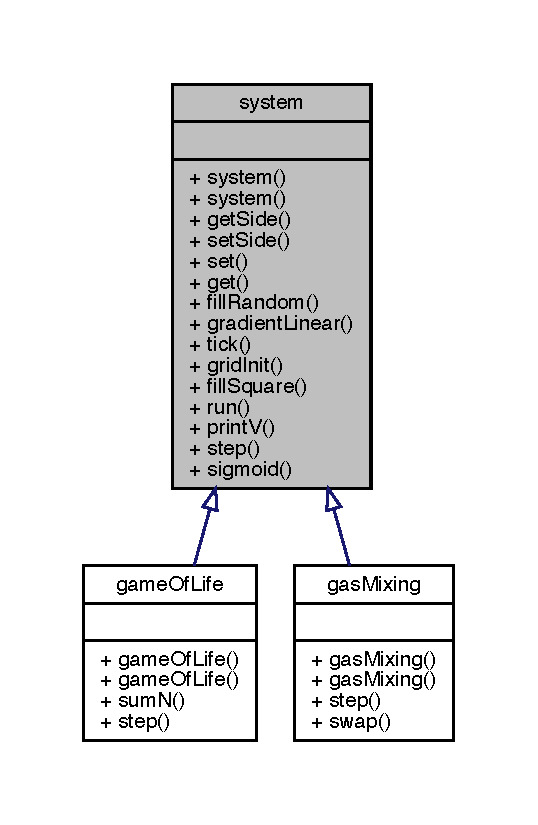
\includegraphics[width=258pt]{classsystem__inherit__graph}
\end{center}
\end{figure}


Collaboration diagram for system\+:
\nopagebreak
\begin{figure}[H]
\begin{center}
\leavevmode
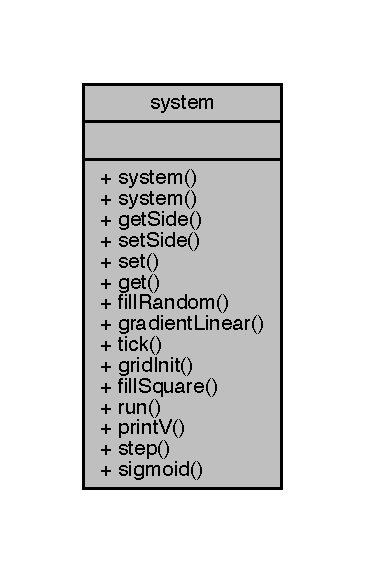
\includegraphics[width=175pt]{classsystem__coll__graph}
\end{center}
\end{figure}
\subsection*{Public Member Functions}
\begin{DoxyCompactItemize}
\item 
\mbox{\Hypertarget{classsystem_a8e1d6ac8f175a0069a3c5cbcbe058ed9}\label{classsystem_a8e1d6ac8f175a0069a3c5cbcbe058ed9}} 
\hyperlink{classsystem_a8e1d6ac8f175a0069a3c5cbcbe058ed9}{system} (void)
\begin{DoxyCompactList}\small\item\em Default constructor. \end{DoxyCompactList}\item 
\mbox{\Hypertarget{classsystem_a1792d5fc1f824113d7852a8f99416495}\label{classsystem_a1792d5fc1f824113d7852a8f99416495}} 
\hyperlink{classsystem_a1792d5fc1f824113d7852a8f99416495}{system} (int side)
\begin{DoxyCompactList}\small\item\em Constructor with system side. \end{DoxyCompactList}\item 
\mbox{\Hypertarget{classsystem_a7480d03afdf71f4e1afc757a323faf6c}\label{classsystem_a7480d03afdf71f4e1afc757a323faf6c}} 
int \hyperlink{classsystem_a7480d03afdf71f4e1afc757a323faf6c}{get\+Side} (void)
\begin{DoxyCompactList}\small\item\em Get side of system\textquotesingle{}s world. \end{DoxyCompactList}\item 
\mbox{\Hypertarget{classsystem_ae139efd3a2598bc297b9224868058d7d}\label{classsystem_ae139efd3a2598bc297b9224868058d7d}} 
void \hyperlink{classsystem_ae139efd3a2598bc297b9224868058d7d}{set\+Side} (int a)
\begin{DoxyCompactList}\small\item\em Set side of system\textquotesingle{}s world. \end{DoxyCompactList}\item 
void \hyperlink{classsystem_a0c16c03ebc2912428bb83ec8310533d3}{set} (int i, int j, int value)
\item 
int \hyperlink{classsystem_a515cbef246f97a9eb89ce36324fee14e}{get} (int i, int j)
\item 
void \hyperlink{classsystem_a774fdf388271bf46bf1125cc186e32d6}{fill\+Random} (\hyperlink{classrandomv}{randomv} \&r, double p)
\item 
void \hyperlink{classsystem_a720cb2d9e63c4ae5a704e912359ad009}{gradient\+Linear} (\hyperlink{classrandomv}{randomv} \&r)
\item 
\mbox{\Hypertarget{classsystem_ada156ed7f1068472dcede241f659a24a}\label{classsystem_ada156ed7f1068472dcede241f659a24a}} 
void \hyperlink{classsystem_ada156ed7f1068472dcede241f659a24a}{tick} ()
\begin{DoxyCompactList}\small\item\em Evolve the system by a single step. \end{DoxyCompactList}\item 
\mbox{\Hypertarget{classsystem_adfc9931a4de3d0fca13773ac86c9c63f}\label{classsystem_adfc9931a4de3d0fca13773ac86c9c63f}} 
void \hyperlink{classsystem_adfc9931a4de3d0fca13773ac86c9c63f}{grid\+Init} (void)
\begin{DoxyCompactList}\small\item\em initialize system world \end{DoxyCompactList}\item 
void \hyperlink{classsystem_ae1cb4d26da7e546b5a6bb1c5b21d1abe}{fill\+Square} (\hyperlink{classrandomv}{randomv} \&r, int window, double p)
\begin{DoxyCompactList}\small\item\em Fill a square region of the environmnet. \end{DoxyCompactList}\item 
void \hyperlink{classsystem_a96961c5218682019c8d1f9f1a01512f1}{run} (int replicate\+ID, int Tmax, \hyperlink{classrandomv}{randomv} \&r, ostream \&sout, ostream \&wout, ostream \&vout, \hyperlink{classentropy}{entropy} \&entropy\+Functions, int byS, int byW, int byV)
\begin{DoxyCompactList}\small\item\em Run the simulation. \end{DoxyCompactList}\item 
void \hyperlink{classsystem_a5536661225ddf0de78c4b81fd8b34978}{printV} (int t, ostream \&vout)
\item 
\mbox{\Hypertarget{classsystem_aab28302f43e7ee42da51eb723f091533}\label{classsystem_aab28302f43e7ee42da51eb723f091533}} 
virtual void \hyperlink{classsystem_aab28302f43e7ee42da51eb723f091533}{step} (\hyperlink{classrandomv}{randomv} \&r)
\begin{DoxyCompactList}\small\item\em Evolve the system by a single step. \end{DoxyCompactList}\item 
double \hyperlink{classsystem_ac4e59474bfe93c5ca7ac46a79d738a4b}{sigmoid} (double L, double k, double x0, double x)
\end{DoxyCompactItemize}


\subsection{Detailed Description}
Abstract system 

Definition at line 13 of file system.\+h.



\subsection{Member Function Documentation}
\mbox{\Hypertarget{classsystem_a774fdf388271bf46bf1125cc186e32d6}\label{classsystem_a774fdf388271bf46bf1125cc186e32d6}} 
\index{system@{system}!fill\+Random@{fill\+Random}}
\index{fill\+Random@{fill\+Random}!system@{system}}
\subsubsection{\texorpdfstring{fill\+Random()}{fillRandom()}}
{\footnotesize\ttfamily void system\+::fill\+Random (\begin{DoxyParamCaption}\item[{\hyperlink{classrandomv}{randomv} \&}]{r,  }\item[{double}]{p }\end{DoxyParamCaption})}

Fill cells in central cell of grid with probability p 
\begin{DoxyParams}[1]{Parameters}
\mbox{\tt in}  & {\em r} & Reference to random class generator \\
\hline
 & {\em p} & Probability of filling cell with value of 1 \\
\hline
\end{DoxyParams}
\begin{DoxyReturn}{Returns}
Nothing 
\end{DoxyReturn}


Definition at line 57 of file system.\+cpp.

\mbox{\Hypertarget{classsystem_ae1cb4d26da7e546b5a6bb1c5b21d1abe}\label{classsystem_ae1cb4d26da7e546b5a6bb1c5b21d1abe}} 
\index{system@{system}!fill\+Square@{fill\+Square}}
\index{fill\+Square@{fill\+Square}!system@{system}}
\subsubsection{\texorpdfstring{fill\+Square()}{fillSquare()}}
{\footnotesize\ttfamily void system\+::fill\+Square (\begin{DoxyParamCaption}\item[{\hyperlink{classrandomv}{randomv} \&}]{r,  }\item[{int}]{window,  }\item[{double}]{p }\end{DoxyParamCaption})}



Fill a square region of the environmnet. 

Fills with 1s a square subregion of the environmnet. 
\begin{DoxyParams}[1]{Parameters}
\mbox{\tt in}  & {\em r} & Instance of random number generator class. \\
\hline
\mbox{\tt in}  & {\em window} & Side of subregion to be filled in. \\
\hline
\mbox{\tt in}  & {\em p} & Probability of filling each cell within subregion. \\
\hline
\end{DoxyParams}
\begin{DoxyReturn}{Returns}
Nothing 
\end{DoxyReturn}


Definition at line 47 of file system.\+cpp.

\mbox{\Hypertarget{classsystem_a515cbef246f97a9eb89ce36324fee14e}\label{classsystem_a515cbef246f97a9eb89ce36324fee14e}} 
\index{system@{system}!get@{get}}
\index{get@{get}!system@{system}}
\subsubsection{\texorpdfstring{get()}{get()}}
{\footnotesize\ttfamily int system\+::get (\begin{DoxyParamCaption}\item[{int}]{i,  }\item[{int}]{j }\end{DoxyParamCaption})}

Get value of cell i,j in systems world 
\begin{DoxyParams}[1]{Parameters}
\mbox{\tt in}  & {\em i} & x-\/axis coordinate. \\
\hline
\mbox{\tt in}  & {\em j} & y-\/axis coordinate. \\
\hline
\end{DoxyParams}
\begin{DoxyReturn}{Returns}
int Value of cell i,j 
\end{DoxyReturn}


Definition at line 39 of file system.\+cpp.

\mbox{\Hypertarget{classsystem_a720cb2d9e63c4ae5a704e912359ad009}\label{classsystem_a720cb2d9e63c4ae5a704e912359ad009}} 
\index{system@{system}!gradient\+Linear@{gradient\+Linear}}
\index{gradient\+Linear@{gradient\+Linear}!system@{system}}
\subsubsection{\texorpdfstring{gradient\+Linear()}{gradientLinear()}}
{\footnotesize\ttfamily void system\+::gradient\+Linear (\begin{DoxyParamCaption}\item[{\hyperlink{classrandomv}{randomv} \&}]{r }\end{DoxyParamCaption})}

Fill the grid with a linear density gradient 
\begin{DoxyParams}[1]{Parameters}
\mbox{\tt in}  & {\em r} & Instance of random number generator class \\
\hline
\end{DoxyParams}
\begin{DoxyReturn}{Returns}
Nothing 
\end{DoxyReturn}


Definition at line 67 of file system.\+cpp.

\mbox{\Hypertarget{classsystem_a5536661225ddf0de78c4b81fd8b34978}\label{classsystem_a5536661225ddf0de78c4b81fd8b34978}} 
\index{system@{system}!printV@{printV}}
\index{printV@{printV}!system@{system}}
\subsubsection{\texorpdfstring{print\+V()}{printV()}}
{\footnotesize\ttfamily void system\+::printV (\begin{DoxyParamCaption}\item[{int}]{t,  }\item[{ostream \&}]{vout }\end{DoxyParamCaption})}

Print state vector of system at cycle t 
\begin{DoxyParams}[1]{Parameters}
\mbox{\tt in}  & {\em t} & The cycle t \\
\hline
\mbox{\tt in}  & {\em vout} & Output stream \\
\hline
\end{DoxyParams}
\begin{DoxyReturn}{Returns}
Nothing 
\end{DoxyReturn}


Definition at line 152 of file system.\+cpp.

\mbox{\Hypertarget{classsystem_a96961c5218682019c8d1f9f1a01512f1}\label{classsystem_a96961c5218682019c8d1f9f1a01512f1}} 
\index{system@{system}!run@{run}}
\index{run@{run}!system@{system}}
\subsubsection{\texorpdfstring{run()}{run()}}
{\footnotesize\ttfamily void system\+::run (\begin{DoxyParamCaption}\item[{int}]{replicate\+ID,  }\item[{int}]{Tmax,  }\item[{\hyperlink{classrandomv}{randomv} \&}]{r,  }\item[{ostream \&}]{sout,  }\item[{ostream \&}]{wout,  }\item[{ostream \&}]{vout,  }\item[{\hyperlink{classentropy}{entropy} \&}]{entropy\+Functions,  }\item[{int}]{byS,  }\item[{int}]{byW,  }\item[{int}]{byV }\end{DoxyParamCaption})}



Run the simulation. 

Performs a simulation run and calculates relevant statistics. 
\begin{DoxyParams}[1]{Parameters}
\mbox{\tt in}  & {\em replicate\+ID} & Replicate ID of simulation. \\
\hline
\mbox{\tt in}  & {\em Tmax} & Run simulations for Tmax steps. \\
\hline
\mbox{\tt in}  & {\em r} & Random number generation class. \\
\hline
\mbox{\tt out}  & {\em sout} & Statistics on three subgrids. \\
\hline
\mbox{\tt out}  & {\em wout} & Statistics on coarse grained grid. \\
\hline
\mbox{\tt out}  & {\em vout} & Output stream of the state of the system for each generation. \\
\hline
\mbox{\tt in}  & {\em byS} & Log sout every byS generations. \\
\hline
\mbox{\tt in}  & {\em byW} & Log wout every byS generations. \\
\hline
\mbox{\tt in}  & {\em byV} & Log vout every byS generations. \\
\hline
\mbox{\tt in}  & {\em entropy\+Functions} & Entropy functions instance \\
\hline
\end{DoxyParams}
\begin{DoxyReturn}{Returns}
Nothing 
\end{DoxyReturn}


Definition at line 89 of file system.\+cpp.

\mbox{\Hypertarget{classsystem_a0c16c03ebc2912428bb83ec8310533d3}\label{classsystem_a0c16c03ebc2912428bb83ec8310533d3}} 
\index{system@{system}!set@{set}}
\index{set@{set}!system@{system}}
\subsubsection{\texorpdfstring{set()}{set()}}
{\footnotesize\ttfamily void system\+::set (\begin{DoxyParamCaption}\item[{int}]{i,  }\item[{int}]{j,  }\item[{int}]{value }\end{DoxyParamCaption})}

Set value of cell i,j in systems world 
\begin{DoxyParams}[1]{Parameters}
\mbox{\tt in}  & {\em i} & x-\/axis coordinate. \\
\hline
\mbox{\tt in}  & {\em j} & y-\/axis coordinate. \\
\hline
\mbox{\tt in}  & {\em value} & Value to set cell i,j. \\
\hline
\end{DoxyParams}
\begin{DoxyReturn}{Returns}
Nothing 
\end{DoxyReturn}


Definition at line 31 of file system.\+cpp.

\mbox{\Hypertarget{classsystem_ac4e59474bfe93c5ca7ac46a79d738a4b}\label{classsystem_ac4e59474bfe93c5ca7ac46a79d738a4b}} 
\index{system@{system}!sigmoid@{sigmoid}}
\index{sigmoid@{sigmoid}!system@{system}}
\subsubsection{\texorpdfstring{sigmoid()}{sigmoid()}}
{\footnotesize\ttfamily double system\+::sigmoid (\begin{DoxyParamCaption}\item[{double}]{L,  }\item[{double}]{k,  }\item[{double}]{x0,  }\item[{double}]{x }\end{DoxyParamCaption})}

Generalized logistic function 
\begin{DoxyParams}[1]{Parameters}
\mbox{\tt in}  & {\em L} & The maximum value of the curve \\
\hline
\mbox{\tt in}  & {\em k} & The steepness of the curve \\
\hline
\mbox{\tt in}  & {\em x0} & The x-\/value of the midpoint \\
\hline
\mbox{\tt in}  & {\em x} & The value for which the function is computed \\
\hline
\end{DoxyParams}
\begin{DoxyReturn}{Returns}
$f(x) = \frac{L}{1 + e^{-k()x-x_0}}$ 
\end{DoxyReturn}


Definition at line 77 of file system.\+cpp.



The documentation for this class was generated from the following files\+:\begin{DoxyCompactItemize}
\item 
src/system.\+h\item 
src/system.\+cpp\end{DoxyCompactItemize}

%--- End generated contents ---

% Index
\backmatter
\newpage
\phantomsection
\clearemptydoublepage
\addcontentsline{toc}{chapter}{Index}
\printindex

\end{document}
